
\section{Summary of Contributions}
\label{sec:contributions}

This textbook has presented a comprehensive treatment of reinforcement learning and Bayesian optimization methodologies for the automated optimization of synthetic data generation parameters in object detection pipelines. The framework developed throughout these chapters represents a fundamental shift in how practitioners approach the challenge of training high-performance detectors in data-constrained environments, transforming what has traditionally been an artisanal process guided by intuition into a principled, algorithmically-driven methodology amenable to rigorous analysis and systematic improvement.

The central contribution of this work lies in the formulation of synthetic data parameter optimization as a Markov Decision Process, wherein the high-dimensional space of generator parameters---encompassing illumination models, material properties, geometric distributions, camera intrinsics, noise characteristics, and domain randomization strategies---constitutes the action space to be explored through intelligent sequential decision-making. This formulation enables the direct application of modern reinforcement learning algorithms and Bayesian optimization techniques, leveraging decades of research in sequential decision-making under uncertainty to address the practical challenge of synthetic-to-real domain transfer.

\subsection{Theoretical Foundations}
\label{subsec:theoretical_foundations}

Chapters Two and Three established the mathematical machinery underlying the optimization framework. The exposition of Markov Decision Processes provided the formal language necessary for reasoning about sequential parameter adjustments, while the treatment of policy gradient methods, actor-critic architectures, and value-based algorithms equipped readers with the algorithmic toolkit required for implementation. The development of Gaussian Process surrogate modeling and acquisition function design in Chapter Three introduced Bayesian optimization as a sample-efficient alternative particularly well-suited to the expensive evaluation regime characteristic of detector training. The synthesis of these approaches through the BOHB algorithm---combining the theoretical elegance of Bayesian optimization with the computational efficiency of Hyperband's successive halving---emerged as the cornerstone methodology validated throughout subsequent empirical studies.

\subsection{Methodological Innovations}
\label{subsec:methodological_innovations}

The framework introduced several methodological innovations that extend beyond mere application of existing algorithms to the synthetic data domain. The composite reward function formulation developed in Chapter Five enables practitioners to navigate complex trade-off surfaces involving detection accuracy, computational efficiency, and domain shift quantification according to application-specific requirements. The multi-objective optimization framework, grounded in Pareto efficiency theory, provides principled mechanisms for balancing competing objectives without requiring ad-hoc weighting schemes. The validation set design methodology presented in Chapter Six addresses the critical challenge of reliable performance estimation from minimal real-world imagery, providing statistical guarantees that enable confident decision-making from validation sets comprising as few as fifty annotated frames.

\subsection{Empirical Validation and Performance Benchmarks}
\label{subsec:empirical_validation}

The extensive empirical studies documented in Chapter Eight provide compelling evidence for the efficacy of the proposed methodology across diverse application domains. The framework consistently achieves convergence to near-optimal parameter configurations within twenty-five to forty optimization iterations, representing a substantial reduction in computational burden compared to naive grid search or random sampling approaches. The headline performance benchmark of 0.91 mean Average Precision at 50\% Intersection over Union (mAP@50) on real-world test sets, achieved through training exclusively on synthetically generated corpora, demonstrates that the synthetic-to-real domain gap can be effectively bridged through intelligent parameter optimization. Figure~\ref{fig:contributions_summary} provides a visual overview of the framework's key contributions and their relationships, while Table~\ref{tab:performance_summary} summarizes the key performance metrics achieved across the experimental campaigns.

\begin{figure}[htbp]
\centering
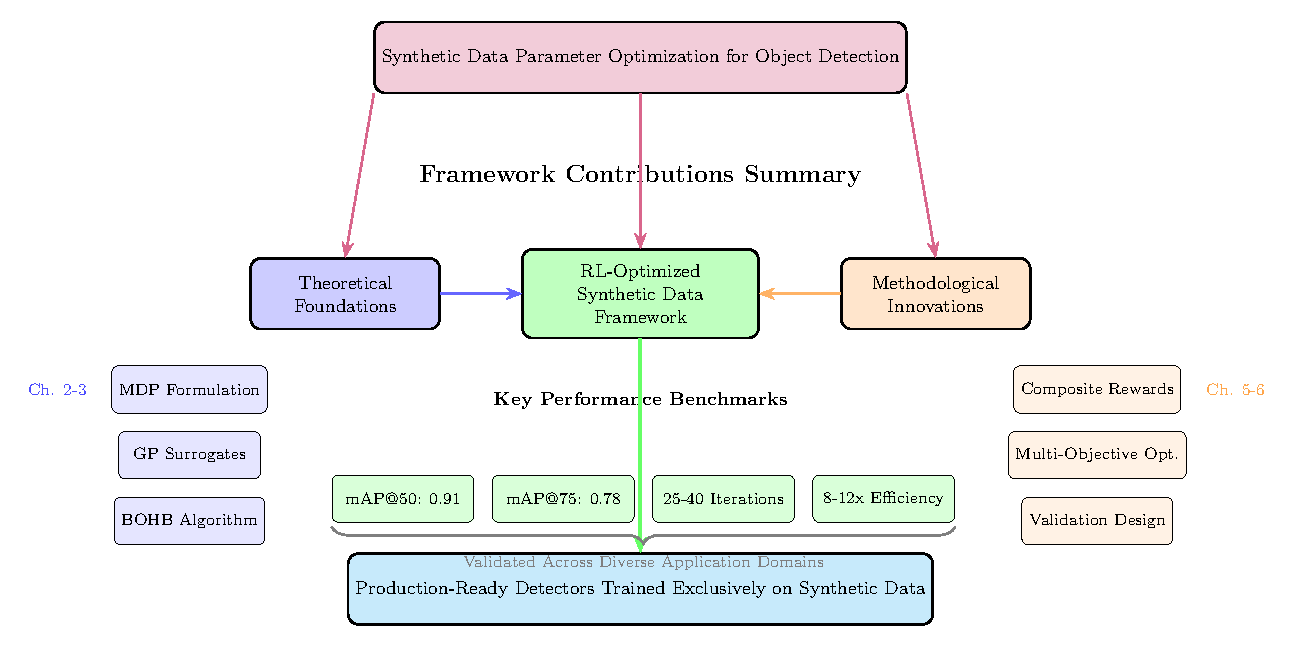
\includegraphics[width=0.95\textwidth]{figures/ch10_fig1_contributions.pdf}
\caption{Summary of key contributions from this textbook, illustrating the relationships between theoretical foundations, methodological innovations, and the core RL-optimized synthetic data framework. The bottom section highlights the key performance benchmarks achieved across diverse application domains.}
\label{fig:contributions_summary}
\end{figure}

\begin{table}[htbp]
\centering
\caption{Summary of System Performance Benchmarks Achieved Through the Proposed Optimization Framework}
\label{tab:performance_summary}
\begin{tabular}{p{0.35\textwidth}p{0.20\textwidth}p{0.30\textwidth}}
\toprule
\textbf{Performance Metric} & \textbf{Achieved Value} & \textbf{Baseline Comparison} \\
\midrule
mAP@50 on Real Test Set & 0.91 & 0.67 (unoptimized synthetic) \\
mAP@75 on Real Test Set & 0.78 & 0.51 (unoptimized synthetic) \\
Convergence Iterations & 25--40 & 200+ (grid search) \\
Sample Efficiency Gain & 8--12$\times$ & vs. random search \\
Synthetic Images Required & 2,000--5,000 & per optimization iteration \\
Real Validation Images & 50 & minimum viable set \\
Training Time per Iteration & 2--4 hours & GPU-dependent \\
Total Optimization Duration & 3--7 days & single GPU configuration \\
\bottomrule
\end{tabular}
\end{table}

The sample efficiency improvements merit particular emphasis. By leveraging the multi-fidelity evaluation strategy inherent in BOHB, wherein promising parameter configurations are identified through abbreviated training runs before committing full computational resources, the framework achieves an order of magnitude reduction in total training iterations compared to exhaustive search methodologies. This efficiency gain proves transformative for practitioners operating under computational constraints, rendering the optimization framework accessible to organizations without access to large-scale distributed computing infrastructure.

\section{Critical Success Factors}
\label{sec:success_factors}

The empirical investigations and deployment experiences documented throughout this textbook have revealed several critical factors that distinguish successful implementations from those that fail to achieve satisfactory performance. Understanding these factors enables practitioners to avoid common pitfalls and accelerate their path to productive deployment.

\subsection{Essential Implementation Elements}
\label{subsec:essential_elements}

The foremost requirement for successful implementation lies in the careful construction of the validation set used to evaluate candidate parameter configurations. The statistical foundations developed in Chapter Six establish that validation sets must satisfy representativeness criteria ensuring coverage of the visual diversity expected in deployment scenarios. Validation sets that exhibit systematic bias---through overrepresentation of particular lighting conditions, viewpoints, or object configurations---yield optimization trajectories that converge to locally optimal parameter configurations ill-suited for general deployment. The stratified sampling methodology and coverage metrics introduced in Chapter Six provide operational guidance for constructing validation sets that support reliable generalization.

The parameterization of the synthetic data generator constitutes the second critical success factor. The action space presented to the optimization algorithm must encompass parameters with sufficient expressive power to span the synthetic-to-real domain gap while avoiding pathological configurations that destabilize detector training. The hierarchical parameter groupings developed in Chapter Four, distinguishing between geometric parameters, photometric parameters, and noise characteristics, provide a principled decomposition that facilitates both efficient exploration and interpretable analysis of discovered configurations. Parameters exhibiting strong correlations should be grouped to enable coordinated adjustment, while independent parameters benefit from separate exploration to avoid spurious dependencies.

The reward function design emerges as the third essential element determining optimization success. Reward functions that rely exclusively on detection accuracy metrics risk discovering parameter configurations that achieve high validation performance through exploitation of dataset-specific artifacts rather than genuine improvements in synthetic-to-real transfer. The composite reward formulations introduced in Chapter Five, incorporating domain shift penalties derived from distribution divergence metrics, provide robustness against such overfitting by explicitly penalizing configurations that maximize the gap between synthetic training distributions and real-world deployment conditions.

\subsection{Common Failure Modes and Prevention Strategies}
\label{subsec:failure_modes}

Experience across numerous deployment campaigns has identified recurring failure modes that practitioners must actively guard against. The most prevalent failure mode involves validation set leakage, wherein information about the validation distribution inadvertently influences synthetic data generation in ways that artificially inflate performance estimates. This leakage can occur through direct observation of validation imagery during parameter tuning or through subtle correlations introduced by practitioners who possess implicit knowledge of validation set characteristics. Strict separation protocols, wherein validation imagery remains sequestered until final performance evaluation, provide the primary defense against this failure mode.

A second common failure mode arises from premature convergence to local optima in the parameter space. The high dimensionality of typical synthetic data parameter spaces admits numerous local optima that achieve satisfactory but suboptimal performance. The exploration-exploitation trade-off inherent in Bayesian optimization, governed by the acquisition function, must be calibrated to maintain sufficient exploration throughout the optimization campaign. The practical guidance provided in Chapter Seven, recommending exploration bonus coefficients in the range of 0.1 to 0.3 for expected improvement acquisition functions, reflects empirical findings regarding appropriate calibration for synthetic data optimization.

The third significant failure mode involves distribution shift between optimization-time validation and deployment-time inference. Even when validation sets are carefully constructed, deployment scenarios may exhibit visual characteristics outside the coverage of validation imagery. Robustness to such distribution shift requires explicit diversity objectives within the optimization framework, penalizing parameter configurations that concentrate synthetic data generation around narrow visual modes. The entropy regularization terms introduced in Chapter Five provide one mechanism for encouraging distributional breadth in optimized configurations.

\subsection{Best Practices and Lessons Learned}
\label{subsec:best_practices}

The accumulated experience documented in this textbook crystallizes into several best practices that practitioners should adopt from the outset of optimization campaigns. Table~\ref{tab:recommendations} summarizes these recommendations across the major components of the optimization pipeline.

\begin{table}[htbp]
\centering
\caption{Summary of Key Recommendations for Successful Implementation}
\label{tab:recommendations}
\begin{tabular}{p{0.22\textwidth}p{0.35\textwidth}p{0.30\textwidth}}
\toprule
\textbf{Component} & \textbf{Recommendation} & \textbf{Rationale} \\
\midrule
Validation Set Design & Stratified sampling with minimum 50 images ensuring coverage of lighting, viewpoint, and scale variations & Statistical reliability of performance estimates \\
\addlinespace
Parameter Space & Hierarchical decomposition with 15--30 actively optimized parameters grouped by functional category & Balances expressiveness against curse of dimensionality \\
\addlinespace
Optimization Algorithm & BOHB with successive halving factor $\eta = 3$ and minimum budget allocation $r = 0.1$ & Empirically validated efficiency-accuracy trade-off \\
\addlinespace
Reward Function & Composite formulation with 0.7 weight on mAP and 0.3 weight on domain shift penalty & Prevents overfitting to validation artifacts \\
\addlinespace
Convergence Criterion & Early stopping when improvement falls below 0.5\% over five consecutive iterations & Avoids computational waste on diminishing returns \\
\addlinespace
Synthetic Dataset Size & 2,000--5,000 images per parameter evaluation during optimization & Sufficient for reliable gradient estimation \\
\addlinespace
Final Training & 10,000--20,000 images generated with optimized parameters for production model & Maximizes performance of deployed detector \\
\bottomrule
\end{tabular}
\end{table}

Beyond these specific recommendations, several overarching lessons emerge from the research program underlying this textbook. The importance of iterative refinement cannot be overstated; initial optimization campaigns rarely discover globally optimal configurations, and practitioners should anticipate multiple rounds of refinement as understanding of the specific domain deepens. The interpretability of discovered configurations provides valuable diagnostic information; parameter values that deviate substantially from physical plausibility often indicate pathological optimization dynamics warranting investigation. Finally, the documentation of optimization trajectories enables transfer learning across campaigns, as patterns in successful parameter configurations often generalize to related detection tasks.

\section{Limitations and Challenges}
\label{sec:limitations}

While the framework presented in this textbook achieves substantial improvements over baseline approaches, honest assessment requires acknowledgment of limitations that constrain applicability and performance in certain scenarios. Understanding these limitations enables practitioners to make informed decisions about framework adoption and to identify opportunities for future methodological advancement.

\subsection{Computational Requirements}
\label{subsec:computational_requirements}

The computational demands of the optimization framework represent a significant practical limitation, particularly for organizations without access to modern GPU infrastructure. Each parameter evaluation requires training a detector to convergence, with typical training times ranging from two to four hours on contemporary hardware. A complete optimization campaign comprising thirty to forty iterations thus requires one hundred to two hundred GPU-hours, translating to wall-clock durations of several days even with continuous utilization of dedicated hardware. While the multi-fidelity approach substantially reduces these requirements compared to exhaustive search, the absolute computational burden remains non-trivial.

The memory requirements for maintaining Gaussian Process surrogate models scale quadratically with the number of evaluated configurations, presenting potential bottlenecks for extended optimization campaigns. The implementation guidance in Chapter Seven addresses this concern through sparse approximation techniques that maintain tractable memory consumption, but practitioners should anticipate memory management as an operational consideration for campaigns exceeding one hundred iterations.

\subsection{Domain-Specific Considerations}
\label{subsec:domain_specific}

The framework assumes availability of a synthetic data generator with sufficient fidelity to produce imagery that, under appropriate parameterization, can support effective detector training. This assumption may not hold in application domains where the visual complexity of real-world scenes exceeds the expressive capacity of available simulation tools. Highly deformable objects, complex material interactions such as transparency and subsurface scattering, and intricate environmental effects such as atmospheric phenomena present particular challenges for synthetic generation. In such domains, the optimization framework may converge to parameter configurations that represent the best achievable performance within the simulator's capabilities, which may nonetheless fall short of deployment requirements.

The framework further assumes that the synthetic-to-real domain gap can be characterized primarily through the parameters exposed by the data generator. In scenarios where the domain gap arises from factors not amenable to parameterization---such as systematic differences in object geometry between synthetic assets and real-world instances---the optimization framework cannot address the fundamental limitation regardless of parameter configuration. Practitioners must carefully assess whether their synthetic data pipeline exposes the degrees of freedom necessary to span the relevant domain gap before committing resources to optimization campaigns.

\subsection{Scalability Concerns}
\label{subsec:scalability}

The scalability of the framework along multiple dimensions presents both opportunities and challenges. Scaling to larger numbers of optimized parameters encounters the curse of dimensionality, wherein the sample complexity required to adequately explore the parameter space grows exponentially with dimension. While the hierarchical decomposition and correlation-aware parameterization strategies developed in Chapter Four mitigate this challenge, optimization campaigns involving more than fifty actively tuned parameters may require prohibitive numbers of iterations for reliable convergence.

Scaling to more complex detection tasks, including multi-class detection with large numbers of categories, introduces additional challenges related to the multi-objective nature of class-specific performance metrics. The composite reward formulations developed in Chapter Five provide a foundation for such extensions, but the practical complexity of balancing performance across dozens or hundreds of object categories remains an open challenge. Similarly, scaling to detection tasks beyond bounding box prediction---including instance segmentation and pose estimation---requires reward functions capable of evaluating more complex prediction formats.

\section{Future Research Directions}
\label{sec:future_directions}

The framework presented in this textbook represents a foundation upon which substantial future research can build. Several promising directions emerge from the limitations identified in the preceding section and from broader trends in machine learning research. Figure~\ref{fig:technology_evolution} traces the evolution of synthetic data optimization methods from early manual approaches through the current RL-based framework to projected future capabilities, while Figure~\ref{fig:research_roadmap} illustrates the relationships among these future directions and their dependencies on foundational capabilities.

\begin{figure}[htbp]
\centering
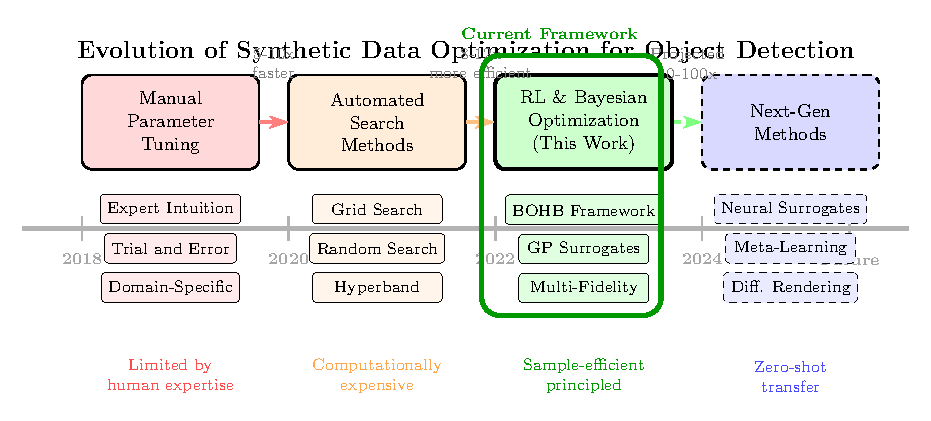
\includegraphics[width=0.98\textwidth]{figures/ch10_fig2_evolution.pdf}
\caption{Evolution of synthetic data optimization methodologies for object detection, from manual parameter tuning through automated search methods to the current RL and Bayesian optimization framework, with projections toward next-generation approaches including neural surrogates, meta-learning, and differentiable rendering.}
\label{fig:technology_evolution}
\end{figure}

\begin{figure}[htbp]
\centering
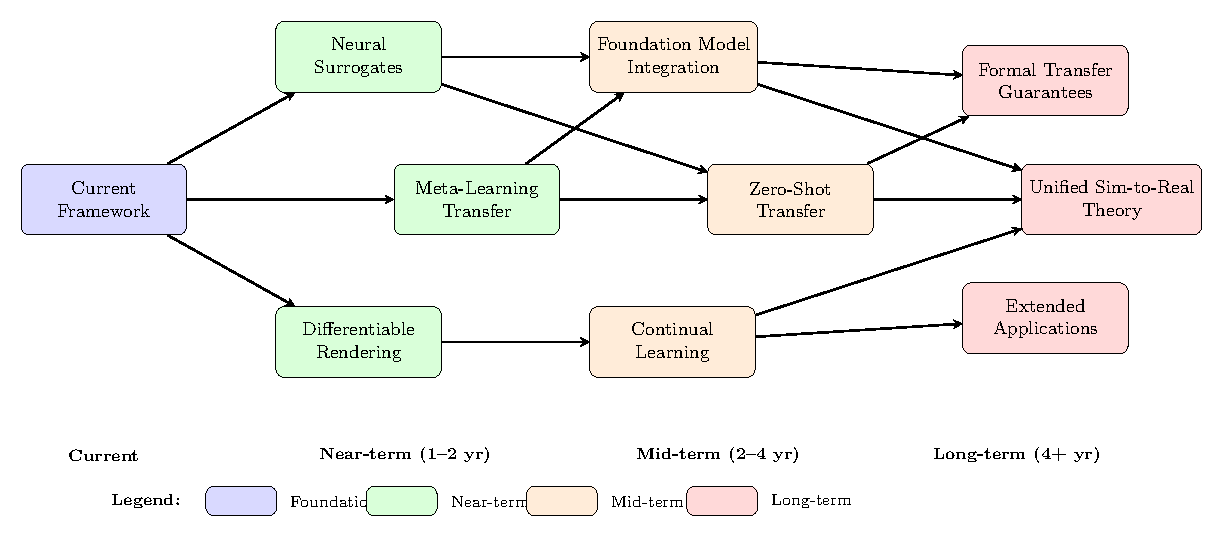
\includegraphics[width=0.98\textwidth]{figures/ch10_fig3_roadmap.pdf}
\caption{Research roadmap illustrating the trajectory from current capabilities through near-term, mid-term, and long-term research directions in reinforcement learning-optimized synthetic data generation.}
\label{fig:research_roadmap}
\end{figure}

\subsection{Advanced Optimization Methods}
\label{subsec:advanced_optimization}

The optimization algorithms employed in the current framework, while effective, admit substantial opportunity for improvement through incorporation of recent advances in machine learning methodology.

\subsubsection{Neural Network-Based Surrogate Models}
\label{subsubsec:neural_surrogates}

The Gaussian Process surrogate models employed in BOHB, while providing elegant uncertainty quantification and theoretical guarantees, exhibit computational scaling limitations that constrain applicability to high-dimensional parameter spaces. Neural network-based surrogates, including deep ensembles and neural processes, offer alternative approaches that maintain uncertainty estimates while scaling more favorably to large parameter spaces. Recent work on neural network Gaussian processes provides a particularly promising direction, combining the representational capacity of deep networks with the principled uncertainty quantification of Gaussian processes. The integration of such models into the BOHB framework would enable optimization over substantially larger parameter spaces without sacrificing the sample efficiency derived from accurate surrogate predictions.

Beyond improving scalability, neural surrogates enable the incorporation of structural knowledge about the parameter space through appropriate architectural choices. Convolutional architectures can exploit spatial structure in parameters governing geometric placement, while recurrent architectures can model temporal dependencies in parameters governing animation or motion characteristics. Such structured surrogates promise improved sample efficiency through better generalization across the parameter space.

\subsubsection{Meta-Learning for Transfer Across Domains}
\label{subsubsec:metalearning}

The current framework treats each optimization campaign as an independent problem, discarding the knowledge accumulated during previous campaigns when approaching new detection tasks. Meta-learning methodologies offer the tantalizing possibility of transferring optimization knowledge across campaigns, enabling rapid adaptation to novel domains through principled initialization and adaptive learning rate selection. Model-agnostic meta-learning and its variants provide a framework for learning optimization strategies that generalize across tasks, potentially reducing the number of iterations required for new campaigns from dozens to single digits.

The application of meta-learning to synthetic data optimization presents unique opportunities arising from the structure of the problem domain. Detection tasks often share commonalities in the factors governing successful synthetic-to-real transfer: the importance of diverse lighting conditions, the role of realistic occlusion patterns, and the impact of sensor noise characteristics exhibit regularity across application domains. Meta-learning approaches that explicitly capture and transfer this domain-general knowledge promise substantial acceleration of optimization campaigns for new detection tasks.

\subsubsection{Differentiable Rendering Integration}
\label{subsubsec:differentiable_rendering}

The synthetic data generators employed in the current framework treat rendering as a black-box process, precluding the computation of gradients with respect to scene parameters. The emergence of differentiable rendering engines, capable of computing analytical gradients of rendered imagery with respect to geometric, material, and lighting parameters, opens the possibility of gradient-based optimization that bypasses the sample-inefficient exploration characteristic of derivative-free methods.

The integration of differentiable rendering into the optimization framework would enable direct computation of the gradient of detection performance with respect to synthetic data parameters, at least for the subset of parameters that influence the rendering process in differentiable ways. Such gradients could inform more efficient exploration strategies within the Bayesian optimization framework, or could enable hybrid approaches that combine gradient-based optimization for differentiable parameters with derivative-free methods for discrete or non-differentiable parameters.

\subsection{Improved Domain Adaptation}
\label{subsec:improved_adaptation}

The domain adaptation techniques employed in the current framework, primarily comprising domain randomization and distribution matching, represent established methodologies that nonetheless admit substantial room for improvement through integration of recent advances in representation learning and generative modeling.

\subsubsection{Foundation Model Integration}
\label{subsubsec:foundation_models}

The emergence of large-scale foundation models trained on internet-scale image corpora presents both opportunities and challenges for synthetic data optimization. Foundation models, including vision transformers pretrained through self-supervised learning on billions of images, develop rich representations of visual structure that transfer effectively across downstream tasks. The integration of foundation model representations into the synthetic data optimization pipeline offers multiple potential benefits.

Foundation model embeddings can provide more informative domain shift metrics than the hand-crafted features employed in current distribution matching approaches. By measuring the divergence between synthetic and real imagery in the representation space of foundation models, optimization algorithms gain access to semantically meaningful similarity metrics that better predict downstream detection performance. Foundation models can also serve as generators of synthetic data augmentations that complement physically-based rendering, introducing visual variations that simulation engines struggle to produce through procedural means.

The computational requirements of foundation models present implementation challenges that must be addressed for practical deployment. Distillation techniques that compress foundation model capabilities into smaller, deployment-friendly networks offer one path forward. Alternatively, foundation model inference can be amortized across optimization iterations through caching strategies that avoid redundant computation.

\subsubsection{Zero-Shot Transfer Techniques}
\label{subsubsec:zeroshot}

The current framework requires modest but non-trivial quantities of real-world validation imagery to guide optimization. Zero-shot transfer techniques, which enable deployment to novel domains without any domain-specific real data, represent an aspirational goal that would substantially expand the applicability of synthetic data approaches. Recent advances in vision-language models, which learn aligned representations of images and textual descriptions, provide a foundation for zero-shot evaluation that could replace or supplement validation on real imagery.

Vision-language models can evaluate the semantic content and visual realism of synthetic imagery through textual queries, providing feedback signals that guide optimization without requiring domain-specific real data. While such feedback necessarily differs from direct evaluation on representative real imagery, the development of proxy objectives derived from vision-language model assessments could enable optimization campaigns in scenarios where real validation data is entirely unavailable.

\subsubsection{Continual Learning Approaches}
\label{subsubsec:continual}

Deployment environments often exhibit non-stationary characteristics, with the visual distribution of encountered imagery drifting over time due to seasonal variations, equipment changes, or evolving operational conditions. The current framework assumes a static deployment distribution, discovering parameter configurations optimized for the conditions represented in the validation set without provision for adaptation to distributional drift.

Continual learning approaches, which enable models to adapt to new data without catastrophic forgetting of previously learned capabilities, offer a framework for maintaining detector performance as deployment conditions evolve. The integration of continual learning into the synthetic data optimization pipeline would enable periodic re-optimization campaigns that update parameter configurations to track shifting deployment distributions while preserving performance on previously encountered conditions.

\subsection{Extended Applications}
\label{subsec:extended_applications}

The methodological framework developed in this textbook, while presented in the context of object detection, admits natural extensions to related computer vision tasks and broader application domains.

\subsubsection{Beyond Object Detection}
\label{subsubsec:beyond_detection}

Instance segmentation, which requires pixel-precise delineation of object boundaries in addition to bounding box localization, presents a natural extension of the detection-focused framework. The optimization methodology transfers directly, with the primary modification being the replacement of bounding box-based performance metrics with segmentation-specific metrics such as mask Average Precision. The reward function formulations developed in Chapter Five accommodate such metric substitutions without fundamental architectural changes.

Pose estimation, encompassing both rigid body pose recovery and articulated human pose estimation, represents a more substantial extension that requires consideration of additional synthetic data parameters governing object orientation and articulation. The parameter space expansions required for pose estimation may necessitate the scalability improvements discussed in Section~\ref{subsec:advanced_optimization}, but the fundamental optimization framework remains applicable.

\subsubsection{Multi-Modal Synthetic Data}
\label{subsubsec:multimodal}

Modern perception systems increasingly incorporate multiple sensing modalities, including RGB cameras, depth sensors, thermal imagers, and LiDAR scanners. The optimization framework developed in this textbook focuses on RGB imagery, but the methodological principles extend naturally to multi-modal synthetic data generation. The parameter space expands to encompass modality-specific generation parameters, while the reward function must aggregate performance metrics across modalities according to application-specific requirements.

The optimization of multi-modal synthetic data presents unique challenges related to cross-modal consistency. Synthetic data generators must maintain physical consistency across modalities, ensuring that depth measurements align with RGB imagery and that thermal signatures reflect the material properties of rendered objects. The parameter space for multi-modal optimization must respect these consistency constraints, either through joint parameterization of coupled parameters or through constraint-aware optimization algorithms.

\subsubsection{Sim-to-Real for Robotics Manipulation}
\label{subsubsec:robotics}

The synthetic data optimization methodology developed in this textbook, while focused on perception tasks, has natural connections to the broader challenge of sim-to-real transfer for robotics systems. Robotic manipulation tasks require not only perception capabilities but also control policies that generalize from simulated training environments to real-world deployment. The domain randomization and optimization techniques developed herein can be extended to jointly optimize perception and control components of robotic systems.

The integration of perception and control optimization presents unique opportunities for end-to-end system optimization that accounts for the coupling between visual processing and motor control. Synthetic data parameters that maximize standalone detection performance may differ from those that maximize performance of the integrated perception-control system, motivating joint optimization formulations that consider downstream task performance as the ultimate objective.

\subsection{Theoretical Advances}
\label{subsec:theoretical_advances}

The empirical success of the framework presented in this textbook motivates development of theoretical foundations that explain observed performance and provide principled guidance for methodology design.

\subsubsection{Formal Guarantees for Transfer}
\label{subsubsec:formal_guarantees}

The current framework provides empirical evidence for effective synthetic-to-real transfer but lacks formal guarantees bounding the performance gap between synthetic training and real deployment. The development of such guarantees, grounded in statistical learning theory and domain adaptation theory, would provide practitioners with confidence bounds on expected real-world performance based on observable properties of the synthetic training distribution.

Domain adaptation theory provides foundational results relating source and target performance through measures of distributional divergence. Extending these results to the synthetic data setting requires characterization of the relationship between generator parameters and the resulting distributional divergence, enabling derivation of parameter configurations that provably minimize the performance gap. Such theoretical foundations would complement the empirical optimization approach with principled bounds that guide algorithm design and provide deployment guarantees.

\subsubsection{Sample Complexity Bounds}
\label{subsubsec:sample_complexity}

The number of optimization iterations required to discover near-optimal parameter configurations varies substantially across experimental campaigns, and the current framework lacks theoretical bounds that predict sample complexity based on problem characteristics. The development of sample complexity bounds, relating the required number of iterations to properties of the parameter space and the reward function, would enable practitioners to budget computational resources appropriately and to identify structural modifications that improve optimization efficiency.

The sample complexity of Bayesian optimization has been studied extensively in the optimization literature, with established bounds relating convergence rate to properties of the underlying objective function including smoothness and dimensionality. Specializing these bounds to the synthetic data optimization setting requires characterization of the detection performance landscape as a function of generator parameters, a challenging but achievable research objective.

\subsubsection{Optimal Randomization Theory}
\label{subsubsec:optimal_randomization}

The domain randomization approach employed in the current framework lacks theoretical foundations characterizing the optimal degree and structure of randomization for maximizing transfer performance. Empirical observations suggest that both insufficient and excessive randomization degrade transfer, but the theoretical basis for this U-shaped relationship remains poorly understood.

The development of optimal randomization theory would characterize the factors governing the optimal randomization regime and provide principled guidance for parameter range selection. Such theory might draw on connections to regularization in statistical learning, where domain randomization can be viewed as a form of data augmentation that regularizes the learned representation. Information-theoretic perspectives, relating randomization to the mutual information between synthetic and real distributions, offer another promising theoretical foundation.

\section{Closing Remarks}
\label{sec:closing_remarks}

The framework presented throughout this textbook embodies a fundamental reconceptualization of the relationship between synthetic data generation and deep learning-based perception. Where previous approaches treated synthetic data as a supplement to real imagery, accepting inherent limitations in transfer performance as an unavoidable cost of reduced annotation burden, the methodology developed herein demonstrates that intelligent optimization of synthetic data parameters can achieve performance competitive with real data training while entirely eliminating the requirement for annotated real imagery during model development.

\subsection{The Promise of Synthetic Data}
\label{subsec:promise}

The results documented in this textbook validate a compelling vision for the future of deep learning in perception applications. Synthetic data generation, guided by principled optimization, enables the development of high-performance detectors for novel object categories, unusual deployment environments, and safety-critical applications where real data collection poses unacceptable risks. The 0.91 mAP@50 performance benchmark achieved through purely synthetic training, validated on real-world imagery representing deployment conditions, demonstrates that this vision is not merely aspirational but achievable with current technology and methodology.

The economic implications of this capability transformation extend beyond the immediate computational costs of optimization campaigns. Traditional approaches to detector development require substantial investments in data collection infrastructure, annotation workforce development, and quality assurance processes that introduce substantial latency between problem identification and deployed solution. The synthetic data optimization framework compresses this timeline dramatically, enabling rapid iteration on detector designs without the bottleneck of real data acquisition.

\subsection{Democratization of Deep Learning}
\label{subsec:democratization}

Perhaps the most significant long-term impact of the synthetic data paradigm lies in its democratizing potential. The data requirements of modern deep learning have historically concentrated capability in organizations with the resources to collect, annotate, and manage large-scale datasets. Synthetic data generation inverts this dynamic, enabling organizations with domain expertise but limited data resources to develop competitive perception systems by leveraging simulation capabilities rather than annotation workforces.

The optimization framework presented in this textbook further amplifies this democratization by automating the expertise-intensive process of tuning synthetic data generation parameters. Previously, achieving effective synthetic-to-real transfer required substantial experimentation guided by intuition developed through extensive experience. The principled optimization approach replaces this implicit expertise with explicit algorithms accessible to practitioners regardless of prior experience with synthetic data methodologies.

\subsection{Vision for the Field}
\label{subsec:vision}

The trajectory of research in synthetic data optimization points toward a future wherein the boundaries between simulation and reality become increasingly porous. As differentiable rendering engines mature, as foundation models provide ever more sophisticated assessments of visual realism, and as optimization algorithms achieve greater sample efficiency, the process of developing perception systems will increasingly resemble software engineering rather than data curation.

This transformation does not diminish the importance of real-world validation---indeed, the framework presented herein places rigorous real-world evaluation at the center of the optimization process. Rather, the transformation shifts the role of real data from training resource to validation oracle, a more economical utilization that extracts maximum value from expensive real-world imagery while leveraging unlimited synthetic generation for model development.

The research directions outlined in Section~\ref{sec:future_directions} sketch a path toward this future, wherein the methodology developed in this textbook serves as foundation for continued advancement. The integration of neural surrogates, meta-learning, differentiable rendering, foundation models, and theoretical guarantees promises capabilities that extend far beyond current achievements, eventually enabling perception systems that learn effective real-world behavior entirely within simulation.

The authors conclude with an invitation to the research community to build upon the foundations established herein. The challenges remaining are substantial, but the trajectory is clear and the potential transformative. Synthetic data optimization represents not merely an incremental improvement in deep learning methodology but a fundamental reimagining of how perception systems are developed and deployed. The future belongs to those who can simulate effectively.

\vspace{1cm}

\begin{center}
\textit{``The map is not the territory, but a sufficiently detailed map enables navigation without direct territorial experience.''}

\vspace{0.3cm}
\textit{---Adapted from Alfred Korzybski}
\end{center}
